\documentclass[titlepage, 11pt]{article}
\usepackage[utf8]{inputenc}     			% UTF8 encoding
\usepackage[margin=1in]{geometry}     		% margins 

\usepackage{hyperref} 						% href
\usepackage{graphicx}
\usepackage[font=small,labelfont=bf]{caption} % Required for specifying captions to tables and figures
\usepackage{verbatimbox}


\title{
	\textbf{Project 1: Movie Recommender System} \\
	Machine learning (CS582), MIU \thanks{Instructor: Anthony Sander}
}

\author{
    Baraa Mousa Noufal \and Ivan Krasowski Bissio
        \and Muzammil Husnain \and Umair Saeed
}
\date{\today}

\begin{document}
\maketitle
\tableofcontents

\begin{abstract}
	\addcontentsline{toc}{section}{Abstract}
	\begin{center}
    \begin{minipage}{0.85\textwidth}
        Machine Learning models are used to predict data of interest using known data as input.
        Recommender Systems are one use-of-case of said models.
        In fact, they are a world of possibilities themselves.
        The goal of this project is to show several possible implementations of a Movie Recommender System,
        including Demographic, Content-based and Collaborative Filtering
        (this one, implemented both with SVD technique and a Neural Network)
        and simulate a production environment were these could be of use, making it as close to reality as possible. 
    \end{minipage}
\end{center}
\end{abstract}

\section{About the Dataset}
The chosen dataset is a mix of two web-available datasets:
\href{https://www.kaggle.com/rounakbanik/the-movies-dataset}{The Movies Dataset}
and \href{https://www.kaggle.com/tmdb/tmdb-movie-metadata}{TMDb 5000 Movie Dataset}.
We opted for these datasets because they give us enough movies with representative information, including ratings from users,
which allows us to develop the three kinds of recommenders we are trying to build.

\subsection{EDA: Exploratory Data Analysis}
\begin{itemize}
	\item The dataset collects multiple features related to each movie, including title, genre, actors, production company and much more. It also provides connection between users and movies through their ratings.
	\item For each movie we hold the data that is important for recommending (since we are experimenting with different combinations, we decide not to drop anything in advance, but to use what we need depending on the project phase).
\end{itemize}

\section{\emph{Trending Now}: Demographic Filtering}
This section presents our work with a demographic filter for recommending top trending movies.
That is, "best" movies in the entire dataset are presented as such.\\
The challenge, precisely, is defining how to say that certain movies are the best.

\subsection*{Metric}
We choose the \emph{weighted average rating}
\footnote{\href{https://math.stackexchange.com/questions/169032/understanding-the-imdb-weighted-rating-function-for-usage-on-my-own-website}{https://math.stackexchange.com/questions/169032/understanding-the-imdb-weighted-rating-function-for-usage-on-my-own-website}}
for assigning a value to each of the movies in our dataset, the same used by \href{https://www.imdb.com/chart/top?ref_=nb\_mv\_3\_chttp}{IMDb}.
\begin{center}
    \(WAR = \left(\frac{v}{v+m} \cdot R\right) + \left(\frac{m}{v+m} \cdot C\right)\)
\end{center}
Being:
\begin{itemize}
    \item v $\Rightarrow$ number of votes for the movie
    \item m $\Rightarrow$ minimum votes required to be listed
    \item R $\Rightarrow$ average rating of the movie
    \item C $\Rightarrow$ mean vote for every movie
\end{itemize}

\subsection*{Implementation}
Implementing this recommender means assigning the described score to each movie entry in the dataset,
then sort them descending by their weighted average score,
and finally take the top 10 movies. They are the 10 trending movies.
\begin{center}
    \captionsetup{type=figure}
    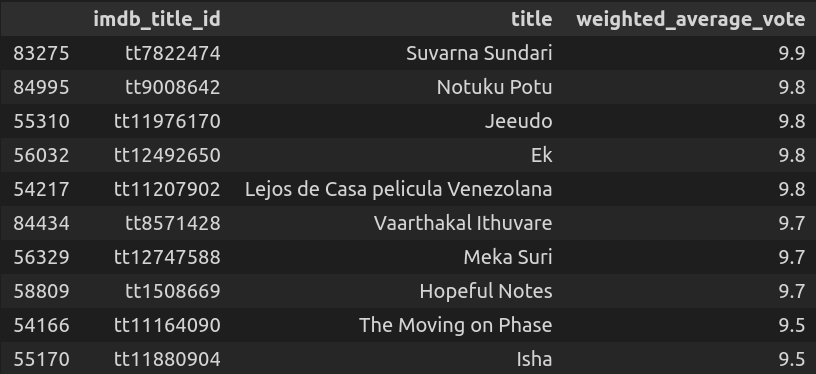
\includegraphics[width=250px]{images/demo-result.png}
    \captionof{figure}{Demographic Filtering Result}
\end{center} 
%TODO: caching?


\section{\emph{Because you watched}: Content-based Filtering}
This section presents our work with a content-based filter for
recommending movies related to another selected movie,
by defining some similarity metric supported by its features.

% get k=10 related movies
% -> get all movies
% -> for each movie, using certain criteria, generate a similarity coefficient (e.g. using cosine similarity)
% -> sort and get top k=10
\subsection*{Comparison}
Selected a movie, we define a similarity function for comparing it with every other movie in the dataset.
We consider two different approaches:
\begin{enumerate}
    \item The description of a movie already tells a lot about it; so, the first approach is taking the description string as the feature to compare (after applying TF-IDF on it).
    \item The second approach is making a "soup" of different features of a movie that we consider relevant for describing it.
\end{enumerate}
For both alternatives, the chosen objects of comparison from both the selected movie and the comparing one are sent as input vectors to a cosine similarity function,
which actually is the distance in polar coordinates for the dot product between both vectors:

\begin{center}
    \( cosine\_similarity = 
        \frac{movie_1 \cdotp movie_2}{\lVert movie_1 \rVert \lVert movie_2 \rVert}
    \)\\
\end{center}

\begin{center}
    \captionsetup{type=figure}
    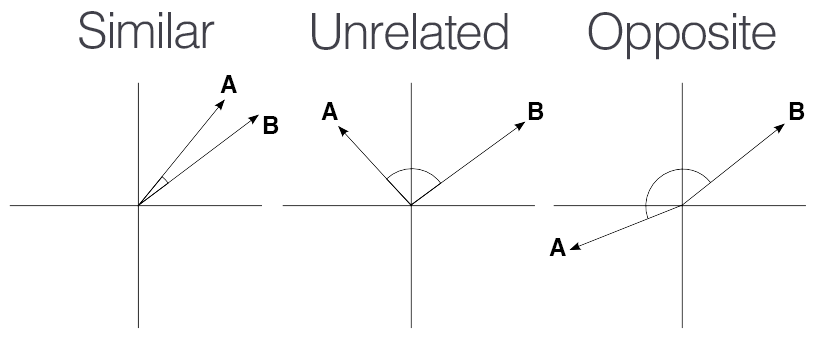
\includegraphics[width=250px]{images/cb-cos.png}
    \captionof{figure}{Graphic Representation of Cosine Similarity}
\end{center}

\subsection*{Implementation}
For a certain movie, we use the Cosine Similarity function between it and every other movie, generating a score for each pair.
Then, we sort them descending by said score, and finally take the top 10 movies. They are the 10 recommended movies, given the first one.
% TODO: show result of the function (image)
% TODO: caching?


\section{\emph{Because of you}: Collaborative Filtering}
This section presents our work with a collaborative filter for
recommending movies for a particular user, given its previous preferences
and the behavior of other users\footnote{Principle: We (people) are not unique}

\subsection{SVD: Singular Value Decomposition}
In linear algebra, the singular value decomposition (SVD) is a factorization of
a real or complex matrix. It generalizes the eigendecomposition of a square normal
matrix with an orthonormal eigenbasis to any {m X n} matrix.
\footnote{\href{https://en.wikipedia.org/wiki/Singular\_value\_decomposition}{https://en.wikipedia.org/wiki/Singular\_value\_decomposition}}\\
In terms of a Movie Recommender System, the SVD decreases the dimension of the utility matrix
by extracting its latent factors (e.g.: age, humour, etc.), and generating an accessible way of
comparing movies and users.\\
\begin{center}
    \captionsetup{type=figure}
    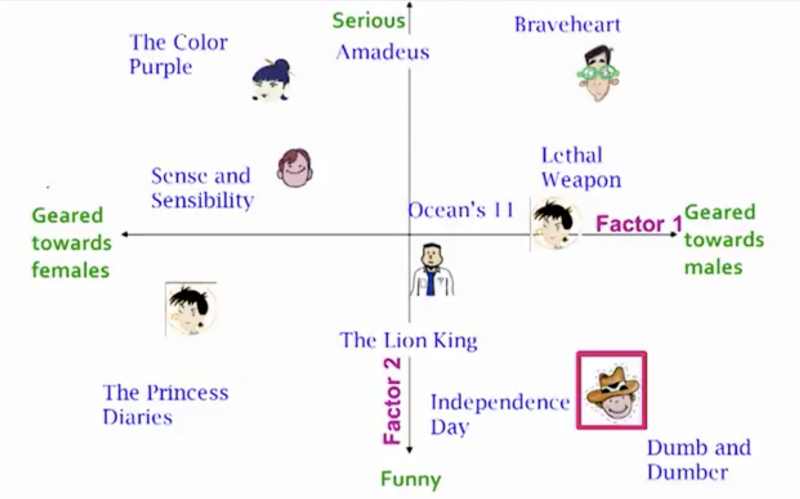
\includegraphics[width=250px]{images/svd-00.png}
    \captionof{figure}{Movie-User simplified-by-SVD comparison}
\end{center}
\subsubsection*{Implementation}
We use the library Surprise\footnote{\href{https://surprise.readthedocs.io/en/stable/matrix\_factorization.html}{https://surprise.readthedocs.io/en/stable/matrix\_factorization.html}}
for implementing our solution. We separate the problem in four different "modules", each one of them represented by a function
and (in most cases) depending on the others:
\begin{enumerate}
    \item Generate SVD model
    \item Predict a score (given a user and a movie)
    \item Get predictions for all movies previously rated in the system (given a user)
    \item Get top predictions
\end{enumerate}
\subsubsection*{Generate Model}
Generating and fitting the model is simplified to us by the library itself.
The cross-validation of training it with our smaller dataset gives us the following results for RSME (Root Mean Square Error) and MAE (Mean Average Error):\\
\begin{center}
    \captionsetup{type=figure}
    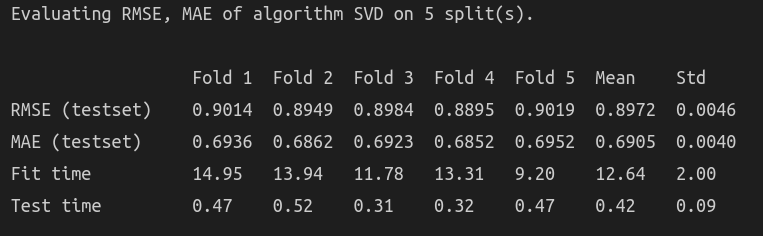
\includegraphics[width=250px]{images/svd-val.png}
    \captionof{figure}{SVD cross-validation}
\end{center}
After making it fit our data, we serialize the generated model using \emph{joblib}
\footnote{\href{https://joblib.readthedocs.io/en/latest/generated/joblib.dump.html}{https://joblib.readthedocs.io/en/latest/generated/joblib.dump.html}},
and from now on we don't need to generate it anymore, but just deserialize it and use it.
\subsubsection*{Predict one score}
Predicting a score involves sending a user and a movie to the SVD model and getting a predicted score (between 1 and 5) for the pair.
For example, asking for the estimate of the score for the movie of id 3 likely given by the user 3 returns us a Prediction object like the following (being \emph{est} the predicted value):
\begin{center}
    \emph{Prediction(uid=3, iid=3, r\_ui=None, est=3.154562267959806, details={'was\_impossible': False})}
\end{center}
\subsubsection*{Predict scores for every movie}
The previous step gives us way to the next one:
if we want to recommend top movies for one user, we can apply the SVD predictor to all rated movies (not by our user) within our dataset
and assign them a potential score for each user-movie pair.
For an increasing dataset, the latter process is batch-intensive, and that's why we use the concurrent.futures\footnote{\href{https://docs.python.org/3/library/concurrent.futures.html}{https://docs.python.org/3/library/concurrent.futures.html}}
Python standard library for running each prediction concurrently.
Applying this process we obtain a list of pairs \emph{(movie id, prediction object)}.
% TODO: talk about caching this list
\subsubsection*{Get top predictions}
Finally, we use this list, order it by prediction value (descending) and take the best 10 movies as our final result.
\begin{center}
    \captionsetup{type=figure}
    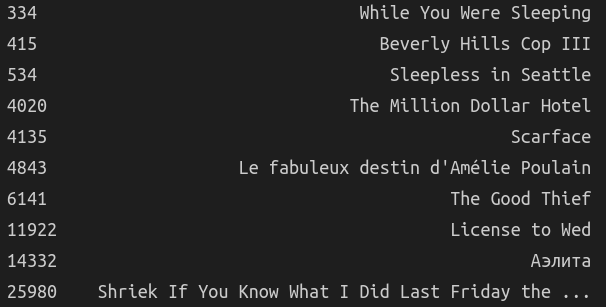
\includegraphics[width=250px]{images/svd-top.png}
    \captionof{figure}{SVD: top 10 predictions for user}
\end{center}

\subsection{Neural Network}
Neural Collaborative filtering attempts to find recommendations similar to those provided by the matrix
factorization on SVD, but powered by the versatility of neural networks.\\
As mentioned previously, we are trying to get a prediction for the score of a movie, for a given user.
That is, we want to feed the model a user and a movie and get a predicted score.\\
\subsubsection*{Network Modeling}
Our Neural Collaborative Filter receives a user and a movie (\emph{Input}) and generates an \emph{Embedding} for each of them.\\
Designing the Neural Network would take much research and experimenting; given our short deadline, we chose to use a tested one
(Wittenauer, 2019\footnote{\href{https://medium.com/@jdwittenauer/deep-learning-with-keras-recommender-systems-e7b99cb29929}{https://medium.com/@jdwittenauer/deep-learning-with-keras-recommender-systems-e7b99cb29929}}).
It involves a sequence of layers and dropouts, following the pattern:
\begin{center}
    \emph{Dropout (5\%) - 10 Fully Connected (FC) Neurons with ReLU activation - Dropout (10\%) - 1 FC Neuron with sigmoid activation - Scaling to prediction range (1-5) = result}\\
\end{center}
\begin{center}
    \captionsetup{type=figure}
    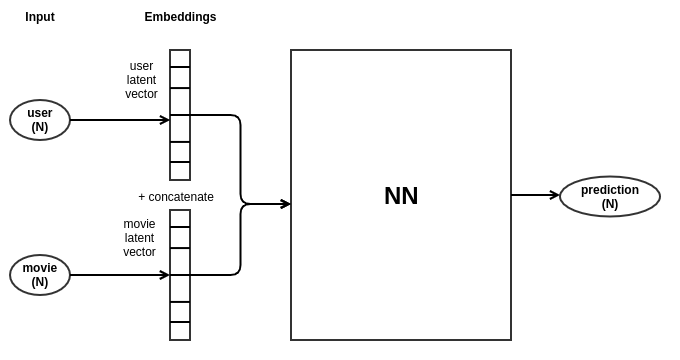
\includegraphics[width=250px]{images/nn-model.png}
    \captionof{figure}{Neural Collaborative Filter Model}
\end{center}

\subsubsection*{Implementation}
For this problem, considering our available time and the high level of abstraction of the library, we decide to use \emph{keras}.
\footnote{\href{https://keras.io/examples/structured\_data/collaborative\_filtering\_movielens/}{https://keras.io/examples/structured\_data/collaborative\_filtering\_movielens/}}
Again, modularizing the problem into functions is the proper solution for us:
\begin{enumerate}
    \item Generate the predictor
    \item Predict scores (given user-movie pairs)
    \item Get top predictions
\end{enumerate}
\subsubsection*{Generate Model}
To generate and train the model we migrate our model directly to the tools provided by keras.
The chosen cost function to optimize is Mean Squared Error.\\
The learning curve obtained by training our small dataset shows a tendency to overfit quickly (after 4 epochs).
Using the large dataset would probably solve this partially, but our resources for this study are limited
and doing so would take over a week (each epoch shows an estimated time of fourteen hours, and 8 epochs are not enough for 26 million inputs)
\begin{center}
    \captionsetup{type=figure}
    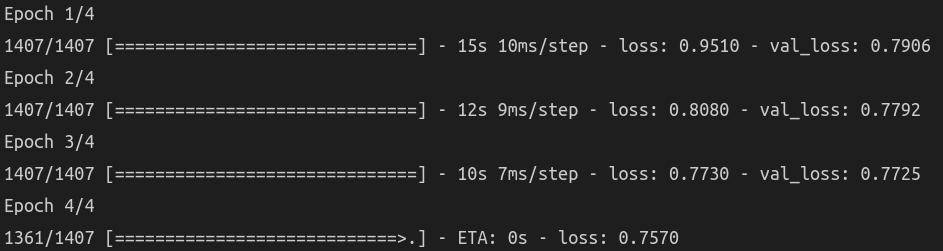
\includegraphics[width=250px]{images/nn-train-sm.png}
    \captionof{figure}{Training the Neural Network}
\end{center}
\begin{center}
    \captionsetup{type=figure}
    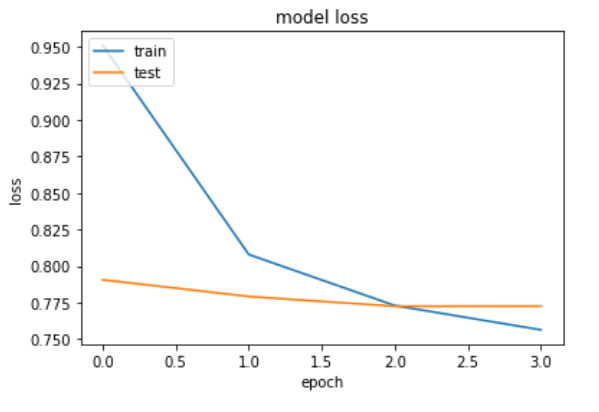
\includegraphics[width=250px]{images/nn-learn.png}
    \captionof{figure}{Learning Curve - Small Dataset}
\end{center}
After making it fit our data, we serialize the generated model using the builtin keras' save() method,
and from now on we don't need to generate it anymore, but just deserialize it and use it.

\subsubsection*{Predict Scores}
Predicting scores involves sending the users and movies lists to the model, and waiting for its answer.

\subsubsection*{Get Top Predictions}
From the nature of the Neural Collaborative Filter, all movies can be sent to the model to get a list of predictions for the same user (sending the user once per movie).\\
Finally, we are able to use this list, order it by prediction value (descending) and take the best 10 movies as our final result.
\begin{center}
    \captionsetup{type=figure}
    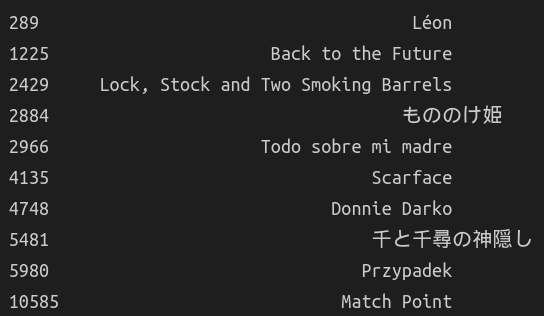
\includegraphics[width=250px]{images/nn-top.png}
    \captionof{figure}{NN: top 10 predictions for user}
\end{center}



\section{In Production}
\subsection{RESTful API}
We choose to expose our developed recommenders using a RESTful API on a web service.
This allows our system to obtain recommendations (all demographic, content-based and collaborative) by sending a request to specific URLs.\\
Here is the part where caching results and serializing the models becomes crucial, given that we want to achieve a quick response time for each request.\\
Since our system has been developed with Python tools, and the language provides good tools (with a broad community) for web development, it seems evident to use it for this services.
We rely on Flask\footnote{\href{https://flask.palletsprojects.com/en/2.0.x/}{https://flask.palletsprojects.com/en/2.0.x/}} library for the task.
\subsection{Docker}
We use Docker\footnote{\href{https://www.docker.com/}{https://www.docker.com/}} for putting our web service in a container,
so to make it platform-independent and don't have to worry about dependencies.
That is, it generates a server itself, exposing the developed API.\\
Our container is available at the DockerHub (\href{https://hub.docker.com/r/barahnofal/cs582-recommender_client}{system} and \href{https://hub.docker.com/r/barahnofal/cs582-recommender_api}{backend})
\subsection{UI}
We use technologies appropriate for User Interface, such as Javascript
\footnote{\href{https://www.javascript.com/}{https://www.javascript.com/}}
and Vue.js\footnote{\href{https://vuejs.org/}{https://vuejs.org/}}\\
By properly structuring our code, we are able to use the implemented web service and,
through it, the recommender models, in order to present them using an interface that is user-friendly:\\
\begin{center}
    \captionsetup{type=figure}
    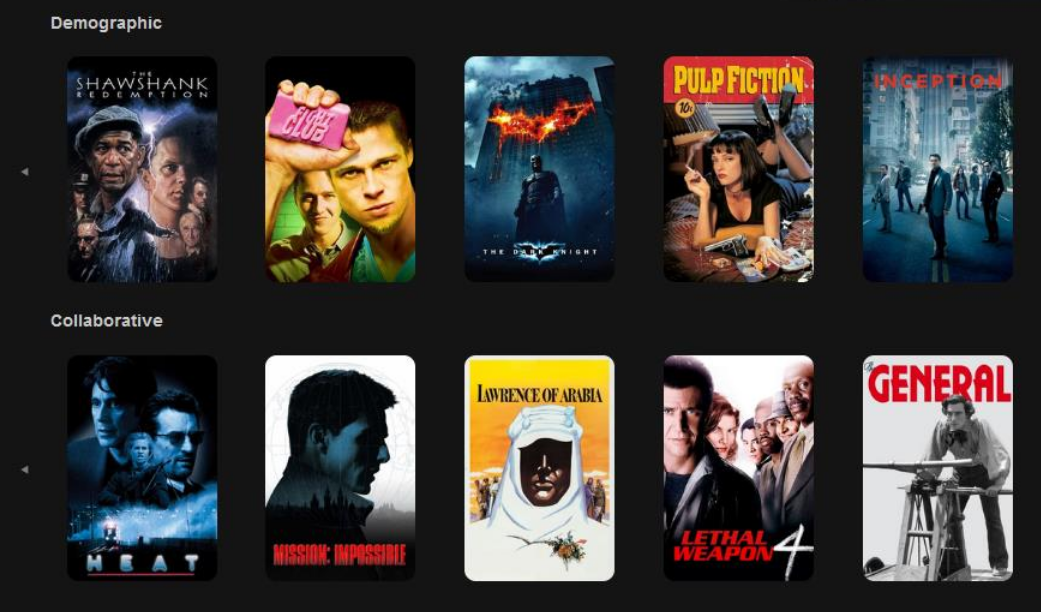
\includegraphics[width=250px]{images/front.png}
    \captionof{figure}{Main Page}
\end{center}

\clearpage
\section{Conclusion}
% Here goes the conclusion

\subsection*{Future Work}
\begin{itemize}
    \item Regarding the Neural Collaborative approach, train the model with a larger dataset, and check whether the layers disposition or the hyperparameters can be tweaked into a better performance.
\end{itemize}

\end{document}
